Resumen de diferentes partes: 
- Librerías utilizadas?? -> LangChain, LangGraph, PgVector

- Ajuste de agentes -> LoRa? -> comentar lo de los agentes instruct.
- El protocolo MCP
- El estado del arte en arquitecturas de agentes LLM y sistemas RAG
- 
- El estado del arte en agentes integrados a proyectos software + contexto de onboarding ~quizás en la introducción.
- Redes neuronales?

2. Agentes LLM (Fundamentos y funcionamiento básico)

¿Qué son los agentes LLM?
2.1. Modelos LLM
2.2. Interacción con herramientas
2.3. Abstracciones en frameworks


\section{Agentes LLM}

Los agentes de Inteligencia Artificial son programas informáticos que implementan modelos computacionales para ejecutar diversas funciones específicas del contexto en el que se aplican. Tras siete décadas y media de investigación, los esfuerzos en el campo se han focalizado en agentes basados en Grandes Modelos de Lenguaje (LLM). 

\subsection{Modelos LLM}

Los LLM son redes neuronales especializadas en el procesamiento del lenguaje natural, basados en la arquitectura Transformer. Esta arquitectura se fundamenta en el mecanismo de atención, el cual transforma la representación del texto para incorporar información contextual de manera escalable al hardware. 

Para comprender el funcionamiento de estos agentes, resulta imprescindible asimilar previamente conceptos como la tokenización y las representaciones vectoriales del lenguaje.

\paragraph{Tokens}
Los tokens constituyen la unidad mínima de texto que el modelo puede procesar. Dado que dichos modelos operan sobre estructuras matemáticas, requieren transformar el lenguaje natural en representaciones matriciales. Para lograr esta conversión, el texto se segmenta en dichas unidades mínimas, que pueden corresponder a caracteres individuales, fragmentos de texto o palabras completas. El conjunto íntegro de estas unidades reconocibles por el modelo configura su vocabulario. 

\paragraph{Representaciones vectoriales}
Constituyen vectores numéricos de dimensionalidad fija que codifican la semántica inherente a cada token. Estos vectores pueden comprender desde 768 dimensiones en arquitecturas como BERT-base hasta superar las 16.000 dimensiones en los modelos más avanzados del estado del arte. Por ejemplo, una dimensión específica podría especializarse en representar conceptos abstractos. En este contexto, la representación vectorial del token ``animal`` contendría un valor más elevado en dicha dimensión que la correspondiente al término ``gato``, reflejando su mayor grado de abstracción conceptual.


\subsection{Interacción con herramientas externas}
Los agentes LLM poseen la capacidad de interactuar con diversas herramientas como búsquedas web\cite{nakano_webgpt_nodate}, bases de datos o interfaces de usuario. Fundamentalmente, un LLM solo genera tokens de texto, por lo que la integración de herramientas se implementa mediante palabras clave que el modelo puede incluir en su salida. Para ello, en el texto de entrada se especifica el esquema de la función a utilizar y, si decide emplearla, el modelo generará el texto correspondiente. Posteriormente, se procesa la respuesta para extraer llamadas a funciones si las hubiese.

La interacción con herramientas es típicamente alternante. Tras realizar la llamada a la herramienta, la salida de esta se utilizará como entrada para el siguiente mensaje del modelo. La figura \ref{fig:herramientas} ilustra el esquema de un agente con acceso a una API del clima. Como el modelo carece de información climática en tiempo real, se le indica en el prompt la posibilidad de invocar esta función. Al incluir la llamada en su texto de salida, se ejecuta la función y su respuesta se transmite al modelo para generar el resultado final.

%xu_rewoo_2023 -> rewoo para no pasar observaciones a react ~orquestar
%react todo
%wang_executable_2024 -> tools con código, igual mejor donde herramientas?


\begin{figure}[H]
  \centering
  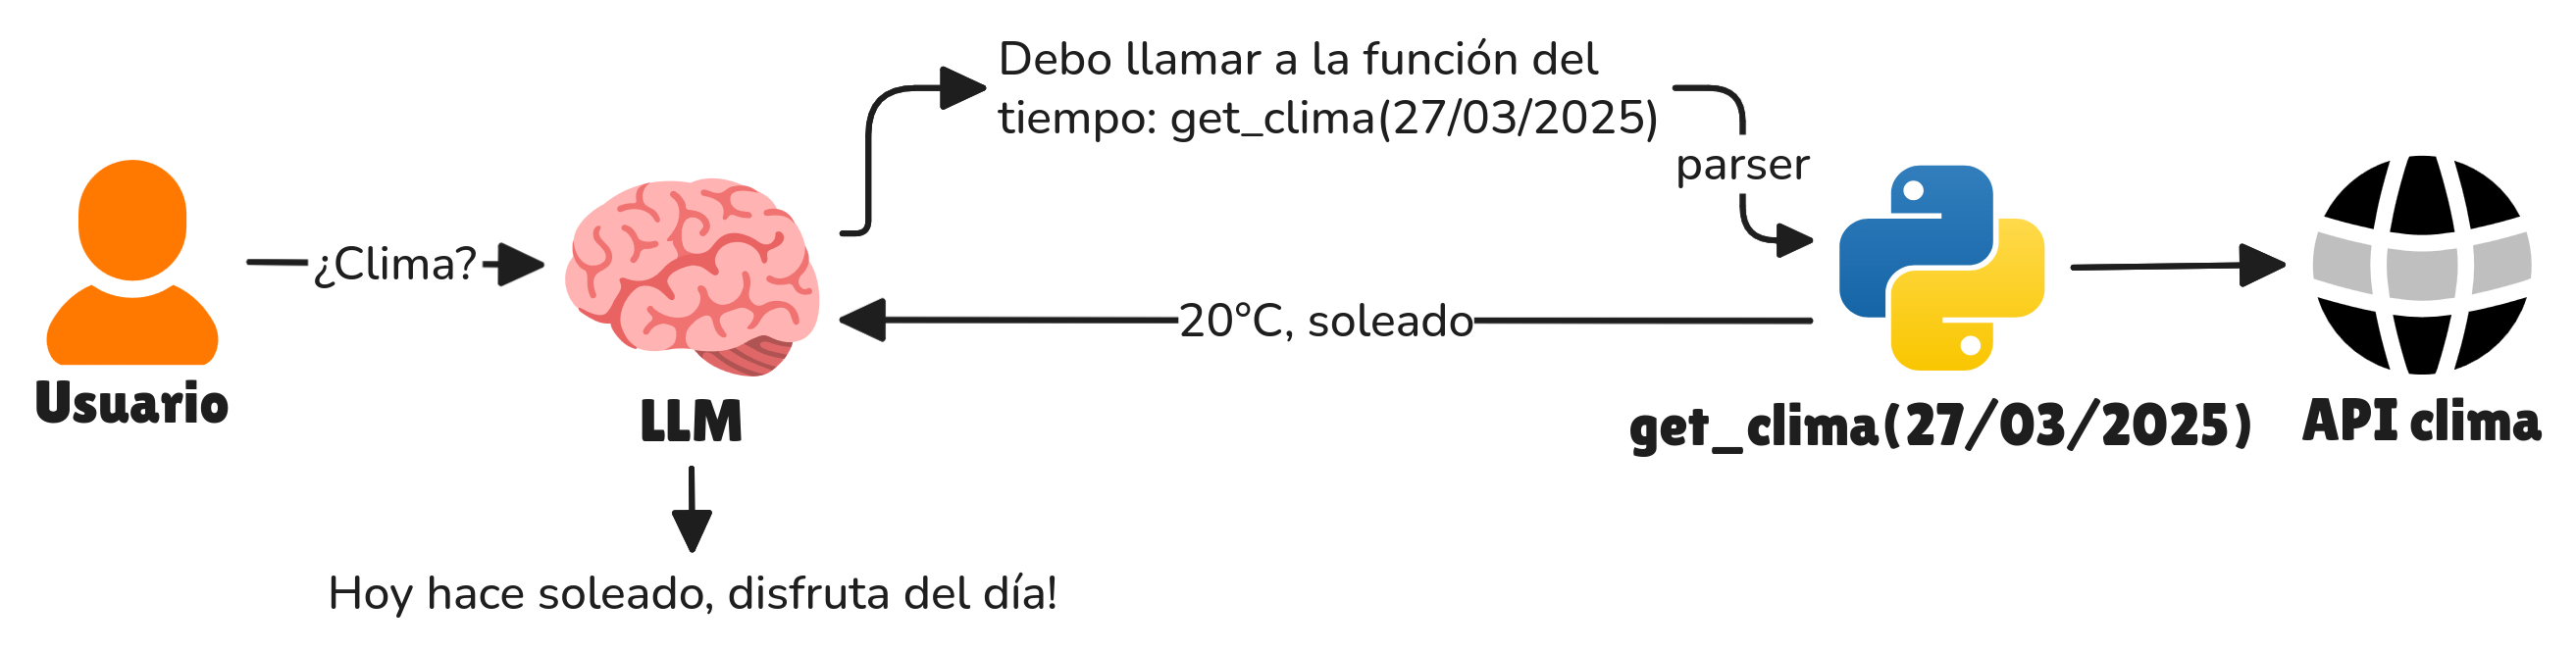
\includegraphics[width=1\linewidth]{figures/herramienta.png}
  \caption{Ejemplo de interacción de un modelo LLM con una herramienta externa.}
  \label{fig:herramientas}
\end{figure}

\subsection{Abstraciones en frameworks}
Aunque los agentes LLM son una tecnología de reciente surgimiento, ya se han desarrollado frameworks que estandarizan su implementación. Estas estructuras de trabajo ofrecen abstracciones de alto nivel para reutilizar funcionalidades comunes presentes en la mayoría de sistemas de agentes.
Las funcionalidades principales que estos frameworks proporcionan son:
\begin{itemize}
\item {\textbf{Gestión de modelos:}} La ejecución de LLM requiere dominio del modelo empleado, ya que cada uno posee tokenizadores específicos y esquemas propios de entrada/salida. Los frameworks ofrecen interfaces unificadas, facilitando el uso de diversos modelos sin conocimientos técnicos precisos.
\item {\textbf{Interacción conversacional:}} La comunicación con los modelos se efectúa mediante un esquema conversacional, donde el modelo recibe un texto de entrada y genera una respuesta correspondiente. Las respuestas y entradas se concatenan secuencialmente para preservar el contexto de la conversación, cada consulta subsiguiente incorpora todos los intercambios precedentes.
  \item {\textbf{Uso de herramientas externas:}} El desarrollador únicamente debe especificar la función que desea incorporar, toda la compljeidad de la interacción se abstrae en el framework.
\item {\textbf{Interacción entre agentes:}} Los agentes pueden establecer comunicación entre sí, permitiendo la construcción de sistemas con mayor complejidad. Algunos frameworks establecen protocolos que definen las modalidades de comunicación entre los distintos agentes.
\end{itemize}

Entre las más populares se encuentran LangChain, LangGraph, LlamaIndex, AutoGen, CrewAI, Smolagents y el reciente OpenAI Agents. 

\section{Model Context Protocol}
todo: referencias a las docs.

El Model Context Protocol (MCP), desarrollado por Anthropic, estandariza la comunicación entre agentes LLM y herramientas. Permite que aplicaciones diversas ofrezcan herramientas a agentes externos sin exponer detalles de implementación. Comparable al modelo OSI, el MCP opera en un nivel de abstracción inferior a los frameworks, proporcionando una capa de interoperabilidad.

La figura \ref{fig:mcp} ilustra el esquema operativo del protocolo. En este contexto, los desarrolladores de Jira y GitHub han implementado un servidor MCP que proporciona las herramientas disponibles al cliente MCP. Este servidor realiza la traducción de las interacciones necesarias con las API de Jira y GitHub, permitiendo que el agente LLM únicamente requiera conocer el esquema funcional que debe utilizar. Por su parte, el cliente MCP se encarga de administrar la comunicación con los diferentes servidores, facilitando que el agente acceda directamente a las herramientas disponibles.

\begin{figure}[H]
  \centering
  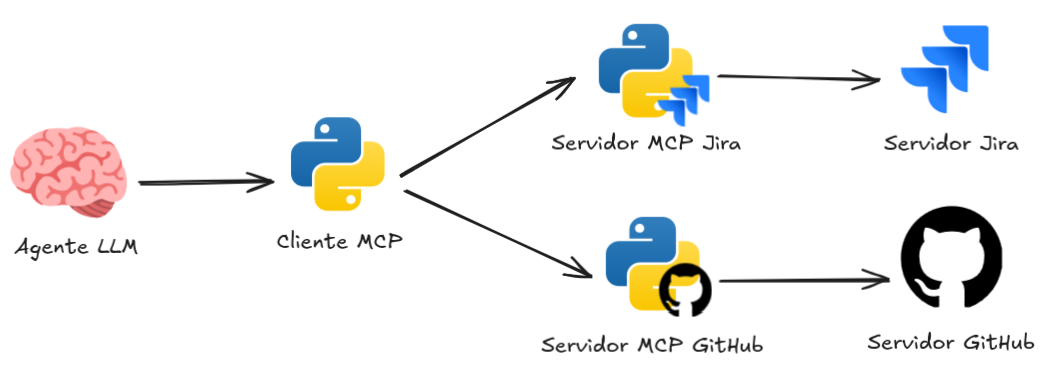
\includegraphics[width=1\linewidth]{figures/mcp.png}
  \caption{Esquema de funcionamiento del Model Context Protocol.}
  \label{fig:mcp}
\end{figure}


El protocolo ofrece dos modos de operación para establecer la comunicación entre cliente y servidor:
\begin{itemize}
  \item{\textbf{Comunicación SSE: } El protocolo Server-Sent Events (SSE) establece un canal de comunicación unidireccional sobre HTTP desde el servidor hacia el cliente. Proporciona actualizaciones en tiempo real con capacidad de streaming. En el protocolo MCP, el cliente efectúa solicitudes para la ejecución de herramientas en el servidor mediante HTTP, a lo que el servidor puede responder mediante eventos SSE.}
\item{\textbf{Comunicación STDIO: } El protocolo de entrada y salida estándar (STDIO) facilita la comunicación bidireccional entre cliente y servidor a nivel de proceso en el sistema operativo. Este mecanismo permite el intercambio de información en formato JSON a través de los canales estándar del sistema. Su diseño, orientado principalmente a entornos locales, restringe la conexión a un único cliente por servidor al limitarse a la comunicación entre dos procesos.}
\end{itemize}
La aplicación de escritorio claude-desktop de Anthropic constituye un reflejo del potencial del protocolo. Esta plataforma ofrece la posibilidad de interactuar con servidores preconfigurados mediante una configuración mínima. Implementando el protocolo STDIO, la aplicación ejecuta los servidores distribuidos por terceros a través del gestor de paquetes UV o Docker. Al incorporar un cliente MCP en la aplicación, consigue integrar las herramientas disponibles en la interfaz de chat con los modelos de Anthropic.

\section{Estado del arte en arquitecturas de agentes LLM}

La comunidad científica ha desarrollado diferentes arquitecturas de agentes para sacar el máximo provecho al rendimiento de los modelos disponibles. Es de destacar la arquitectura RAG, la cual complementa la entrada del modelo con la recuperación de documentos relevantes. Por otro lado, se han realizado diversos esfuerzos en investigar diferentes arquitecturas de comunicación, estrategias de planning o sistemas de memoria, entre otros.

\subsection{Arquitectura RAG}

Los modelos LLM poseen un conocimiento restringido a los datos con los que fueron entrenados. Para superar esta limitación, la arquitectura RAG (Retrieval-Augmented Generation) complementa la generación del LLM mediante la recuperación de información relevante desde repositorios de conocimiento externos. La figura \ref{fig:rag} ilustra un ejemplo de su funcionamiento.    

\begin{figure}[H]
  \centering
  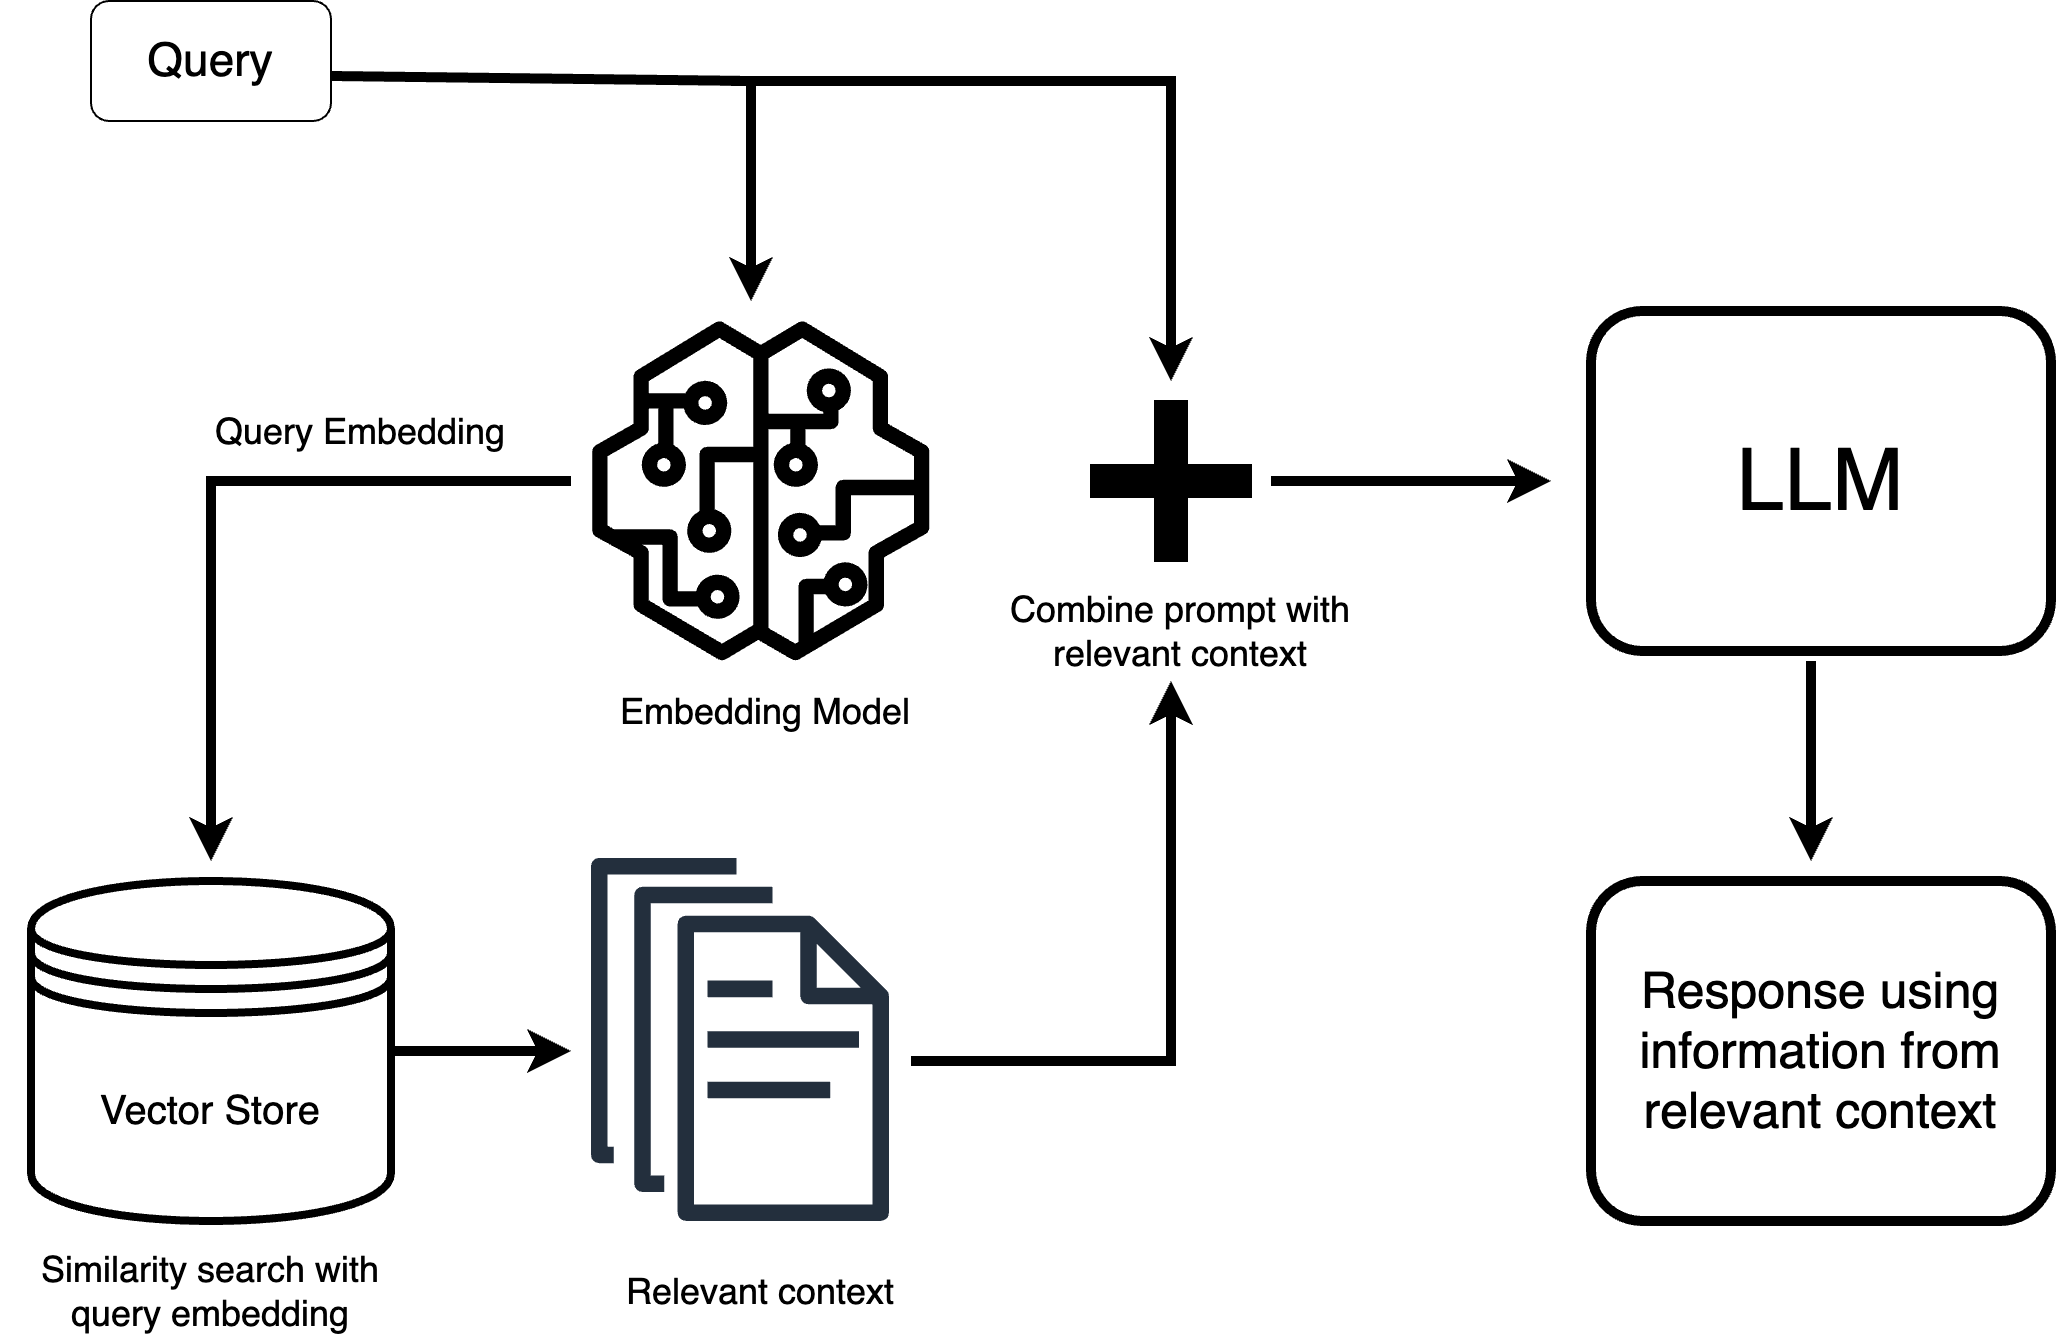
\includegraphics[width=0.5\linewidth]{figures/RAG.png}
  \caption{Esquema de funcionamiento de la arquitectura RAG en un LLM \href{https://www.clarifai.com/blog/what-is-rag-retrieval-augmented-generation}{Fuente}.}
  \label{fig:rag}
\end{figure}

La recuperación de documentos relevantes se puede implementar mediate recuperadores dispersos: expresiones regulares, búsqueda de trigramas [ref], palabras clave, entre otras. No obstante, el enfoque predominante consiste en el uso de recuperadores densos, conocidos como indexación vectorial. En este método, los documentos se transforman en vectores, generalmente mediante LLMs especializados en codificación, denominados Embedders. Al representar los documentos en un espacio vectorial, es posible recuperar aquellos semánticamente más pertinentes mediante la comparación del vector de consulta con los vectores de los documentos indexados, utilizando métricas como la distancia coseno.

\subsubsection{Estrategias RAG avanzadas}
La optimización del rendimiento en arquitecturas RAG ha sido objeto de extensa investigación\cite{zhu_retrieving_2021}\cite{gao_retrieval-augmented_2024}, centrándose en cuatro áreas fundamentales: procesado de documentos, sistemas de recuperación, generación y optimización del pipeline general:
\begin{itemize}
  \item {\textbf{Procesado de documentos:}} La calidad de la indexación documental determina la eficacia del sistema. Entre las estrategias destacadas figuran la eliminación de ruido textual, el ajuste dimensional de chunks y el sistema overlapping window, que superpone fragmentos para preservar la información limítrofe. 
  
  Se han desarrollado también técnicas generativas para mejorar la calidad documental, desde la recuperación de contenidos directamente generados\cite{yu_generate_2023}, la recitación de evidencias\cite{sun_recitation-augmented_2023}, hasta el uso de documentos generados a partir de la query para localizar información relevante\cite{gao_precise_2023}. Estas técnicas pueden complementarse con algoritmos como beam search para incrementar su efectividad\cite{cheng_lift_nodate}\cite{cho_improving_2023-1}\cite{yoran_answering_2024}.
  
  \item {\textbf{Sistemas de recuperación:}} Los recuperadores densos se clasifican en tres categorías: basados en representaciones (ilustrados en la figura \ref{fig:rag}); basados en interacción, que emplean LLM embedders para codificar documentos junto con la consulta, evaluando su relevancia mediante clasificadores densos\cite{ma_query_nodate}\cite{levine_standing_2022}; y enfoques híbridos que combinan ambas estrategias, filtrando inicialmente por representaciones y refinando posteriormente mediante técnicas de interacción\cite{khattab_relevance-guided_2021}. Adicionalmente, existen métodos para condensar la información recuperada, minimizando así la ventana contextual de los generadores \cite{khattab_baleen_nodate}\cite{xu_recomp_2023}.
  
  \item {\textbf{Optimización del pipeline y generación:}} Para tareas que requieren reflexión documental, se han propuesto sistemas de salto múltiple que alternan entre recuperación y generación\cite{shao_enhancing_2023}\cite{qi_answering_2021}\cite{zheng_take_2024}\cite{trivedi_interleaving_2023}. El framework DSP\cite{khattab_demonstrate-search-predict_2023} constituye el referente en sistemas de pregunta-respuesta, utilizando demostraciones para entrenar tanto el extractor como el generador, alternando posteriormente entre búsqueda y predicción. Adaptive RAG\cite{jeong_adaptive-rag_2024} propone clasificar previamente las consultas según su complejidad para determinar la ejecución del proceso, mientras que otros enfoques integran modelos de tamaño reducido para tareas específicas como el resumen\cite{ma_large_2023}.
\end{itemize}

Adicionalmente, el ajuste fino de modelos para tareas RAG específicas mejora significativamente el rendimiento, ya sea optimizando embedders\cite{xiong_approximate_2020}, sistemas de extracción\cite{khattab_relevance-guided_2021}\cite{izacard_atlas_2022}, generación\cite{asai_self-rag_2024}\cite{krishna_rankgen_2022} o reescritura de consultas\cite{ma_query_nodate}. Diversos trabajos han ajustado extractores para LLMs de caja negra\cite{yu_augmentation-adapted_2023}\cite{shi_replug_2023}\cite{lin_ra-dit_2024}\cite{yang_prca_2023}, mientras otros enfoques modifican la arquitectura interna del modelo para incorporar contexto de documentos relevantes durante la generación\cite{guu_realm_2020}.


%lazaridou_internet-augmented_2022 -> rag con internet
%cheng_uprise_2023 -> rag sobre prompts

%li_structure-aware_2023 -> datos estructurados aprender a lenguaje natural


%kang_knowledge_2023 -> combinar RAG con GNN para relaciones 

\subsection{Arquitecturas de interacción entre agentes}
La interacción entre agentes LLM constituye un campo de investigación activo, distinguiéndose diversos avances en módulos de memoria, planificación e interacción multiagente\cite{wang_survey_2024}.
\begin{itemize}
\item{\textbf{Módulos de memoria}}: La investigación abarca memoria conversacional, a corto y largo plazo, cada una con distintos niveles de detalle\cite{zhang_building_2024}. Estas memorias almacenan desde interacciones previas hasta objetivos y registros de eventos\cite{fischer_reflective_2023}\cite{liang_unleashing_2023}, siendo frecuentemente accedidas mediante RAG\cite{zhao_expel_2024}.

La transición entre memorias se define mediante reglas de olvido similares a las humanas\cite{zhong_memorybank_2024}, y su acceso se condiciona por métricas como importancia o recencia\cite{wang_survey_2024}. Generative Agents\cite{park_generative_2023} implementa estas estrategias para simular ecosistemas de NPCs que, almacenando memorias de variada importancia, generan interacciones narrativas complejas.
\item{\textbf{Planificación}}: Los mecanismos de planificación potencian el razonamiento de los agentes sobre sus acciones. Estrategias como la reflexión\cite{shinn_reflexion_nodate}\cite{shinn_reflexion_nodate}\cite{madaan_self-refine_nodate}\cite{miao_selfcheck_2023}, self-consistency\cite{liang_unleashing_2023} o tree of thought\cite{yao_tree_nodate}\cite{wang_recmind_2024} optimizan el razonamiento, aunque modelos recientes como o1 incorporan estas capacidades nativamente.

La estructuración de acciones a realizar es una práctica extendida, definiendo planes de alto nivel que luego se desglosan en acciones específicas\cite{lin_swiftsage_nodate}\cite{huang_language_nodate}\cite{wang_describe_2024}\cite{zhu_ghost_2023}\cite{song_llm-planner_2023}. Las interdependencias entre acciones permiten verificar la validez de los planes generados\cite{raman_planning_nodate}\cite{liu_llmp_2023}\cite{dagan_dynamic_2023}.
Voyager integra memoria y planificación mediante anotación de acciones\cite{wang_voyager_2023}, aprendiendo a interactuar con el entorno como alternativa al aprendizaje por refuerzo. Odyssey perfecciona este enfoque ajustando los modelos con información contextual\cite{liu_odyssey_2024}.
\item{\textbf{Interacción entre agentes: }}El despliegue de agentes especializados coordinados por un router constituye una estrategia para optimizar la precisión con diversas fuentes de datos\cite{karpas_mrkl_2022}\cite{ge_openagi_nodate}.

Enfoques alternativos proponen la interacción directa entre agentes especializados como mecanismo de retroalimentación\cite{zhuge_mindstorms_2023}\cite{du_improving_nodate}. En este ámbito destaca ChatDev\cite{qian_chatdev_2024}, que aborda problemas de ingeniería de software mediante la colaboración de agentes programadores, testers y gestores. MetaGPT\cite{hong_metagpt_2024} refina esta propuesta estableciendo un protocolo de comunicación publisher/subscriber entre agentes, permitiéndoles seleccionar los destinatarios de su información.
\end{itemize}

%todo en capitulo agente código:
%rana_sayplan_2023 -> robot con path de la casa -> similar a repo
%gramopadhye_generating_2023 -> mejora al anterior con few shots entorno



















